\documentclass[a4paper,14pt]{extreport}
\usepackage[left=1.5cm,right=1.5cm,
    top=1.5cm,bottom=2cm,bindingoffset=0cm]{geometry}
\usepackage{scrextend}
\usepackage[T1,T2A]{fontenc}
\usepackage[utf8]{inputenc}
\usepackage[english,russian,ukrainian]{babel}
\usepackage{tabularx}
\usepackage{amssymb}
\usepackage{color}
\usepackage{amsmath}
\usepackage{mathrsfs}
\usepackage{listings}
\usepackage{graphicx}
\graphicspath{ {./images/} }
\usepackage{lipsum}
\usepackage{xcolor}
\usepackage{hyperref}
\usepackage{tcolorbox}
\usepackage{tikz}
\usepackage[framemethod=TikZ]{mdframed}
\usepackage{wrapfig,boxedminipage,lipsum}
\mdfdefinestyle{MyFrame}{%
linecolor=blue,outerlinewidth=2pt,roundcorner=20pt,innertopmargin=\baselineskip,innerbottommargin=\baselineskip,innerrightmargin=20pt,innerleftmargin=20pt,backgroundcolor=gray!50!white}
 \usepackage{csvsimple}
 \usepackage{supertabular}
\usepackage{pdflscape}
\usepackage{fancyvrb}
%\usepackage{comment}
\usepackage{array,tabularx}
\usepackage{colortbl}
\usepackage{fp}

\usepackage{varwidth}
\tcbuselibrary{skins}
\usepackage{fancybox}


\usepackage{tikz}
\usepackage[framemethod=TikZ]{mdframed}
\usepackage{xcolor}
\usetikzlibrary{calc}
\makeatletter
\newlength{\mylength}
\xdef\CircleFactor{1.1}
\setlength\mylength{\dimexpr\f@size pt}
\newsavebox{\mybox}
\newcommand*\circled[2][draw=blue]{\savebox\mybox{\vbox{\vphantom{WL1/}#1}}\setlength\mylength{\dimexpr\CircleFactor\dimexpr\ht\mybox+\dp\mybox\relax\relax}\tikzset{mystyle/.style={circle,#1,minimum height={\mylength}}}
\tikz[baseline=(char.base)]
\node[mystyle] (char) {#2};}
\makeatother

\definecolor{ggreen}{rgb}{0.4,1,0}
\definecolor{rred}{rgb}{1,0.1,0.1}
\definecolor{amber}{rgb}{1.0, 0.75, 0.0}
\definecolor{babyblue}{rgb}{0.54, 0.81, 0.94}
\definecolor{amethyst}{rgb}{0.6, 0.4, 0.8}

\usepackage{float}
\usepackage{wrapfig}
\usepackage{framed}
%for nice Code{
\lstdefinestyle{customc}{
  belowcaptionskip=1\baselineskip,
  breaklines=true,
  frame=L,
  xleftmargin=\parindent,
  language=C,
  showstringspaces=false,
  basicstyle=\small\ttfamily,
  keywordstyle=\bfseries\color{green!40!black},
  commentstyle=\itshape\color{purple!40!black},
  identifierstyle=\color{blue},
  stringstyle=\color{orange},
}
\lstset{escapechar=@,style=customc}
%}


\begin{document}
\pagecolor{white}

%----------------------------------------1
\newtcbox{\xmybox}[1][red]{on line, arc=7pt,colback=#1!10!white,colframe=#1!50!black, before upper={\rule[-3pt]{0pt}{10pt}},boxrule=1pt, boxsep=0pt,left=6pt,right=6pt,top=2pt,bottom=2pt}



\begin{titlepage}
  \begin{center}
    \large
    Національний технічний університет України \\ "Київський політехнічний інститут імені Ігоря Сікорського"


    Факультет Електроніки

    Кафедра мікроелектроніки
    \vfill

    \textsc{ЗВІТ}\\

    {\Large Про виконання лабораторної роботи №6\\
      з дисципліни: «Твердотільна електроніки-1»\\[1cm]

      «ІНТЕГРАЛЬНІ СХЕМИ СТАТИЧНОЇ ЛОГІКИ НА МДН – ТРАНЗИСТОРАХ» \\

    }
  \bigskip
\end{center}
\vfill

\newlength{\ML}
\settowidth{\ML}{«\underline{\hspace{0.4cm}}» \underline{\hspace{2cm}}}
\hfill
\begin{minipage}{1\textwidth}
Виконавець:\\
Студент 3-го курсу \hspace{4cm} $\underset{\text{(підпис)}}{\underline{\hspace{0.2\textwidth}}}$  \hspace{1cm}А.\,С.~Мнацаканов\\
\vspace{1cm}

Превірив: \hspace{6.1cm} $\underset{\text{(підпис)}}{\underline{\hspace{0.2\textwidth}}}$  \hspace{1cm}Л.\,М.~Королевич\\

\end{minipage}

\vfill

\begin{center}
2021
\end{center}
\end{titlepage}
%---------------------------------------------------------------------------------------------------------------------------------------------------------------------------------



\begin{center}1. МЕТА РОБОТИ\\ \end{center}

Дослідження характеристик керуючого транзистора та властивостей
базових інверторів інтегральних схем виготовлених за МДН-технологією.

\begin{center}2. ЗАВДАННЯ\\ \end{center}

2.1 Виконати вимірювання сімейства вихідних вольт-амперних характеристик керуючого інтегрального МДН-транзистора $T_{y}-$ залежності струму стоку від напруги сток-виток. Побудувати сімейство характеристик $I_{c}=I_{c}\left(U_{c c}\right)[$ при $\left.U_{3}=\mathrm{const}\right]$ на одному малюнку.\\

2.2 Визначити крутизну, динамічний опір стоку, коефіцієнт підсилення напруги
- для крутої і для пологої областей вихідних характеристик транзистора $\left(S_{1} ;\right.$ $\left.S_{2} ; r_{c_l} ; r_{c_2} ; \mu_{1} ; \mu_{2}\right)$\\

2.3 Виміряти передавальні характеристики інтегрального МДН-інвертора при різних $\quad$ видах навантаження: \\

\hspace{1cm} а) лінійний резистор $R_{n}$\\

\hspace{1cm} б) МДН-транзистор $T_{y}$ ідентичний керуючому,\\

\hspace{1cm} в) МДН-транзистор з довгим та вузьким каналом $T_{n} .$\\

2.4 Побудувати на одному малюнку графіки передавальних характеристик Знятих $\quad$ для $\quad$ трьох типів інверторів. Визначити коефіцієнти передачі для різних видів навантажень.\\

2.5 За результатами вимірювань побудувати на сімействі вихідних ВАХ керуючого транзистора навантажувальні характеристики для трьох типів навантаження: $R_{n}, T_{y}, T_{n}$\\


2.6 Виконати порівняльний аналіз досліджуваних схем інверторів і зробити висновки про доцільність використання розглянутих типів навантаження в схемах статичної логіки.\\

2.7 Намалюйте можливу структуру одного із досліджених інтегральних МДНінверторів (найоптимальнішого). Запропонуйте заходи щодо зниження порогової напруги та зменшення паразитних ємностей інтегрального МДН інвертора.\\



\newpage
\begin{center}2.1. СХЕМА ДЛЯ ДОСЛІДЖЕННЯ ВОЛЬТ-АМПЕРНОЇ ХАРАКТКРИСТИКИ\\ \end{center}

\begin{figure}[h]
\center{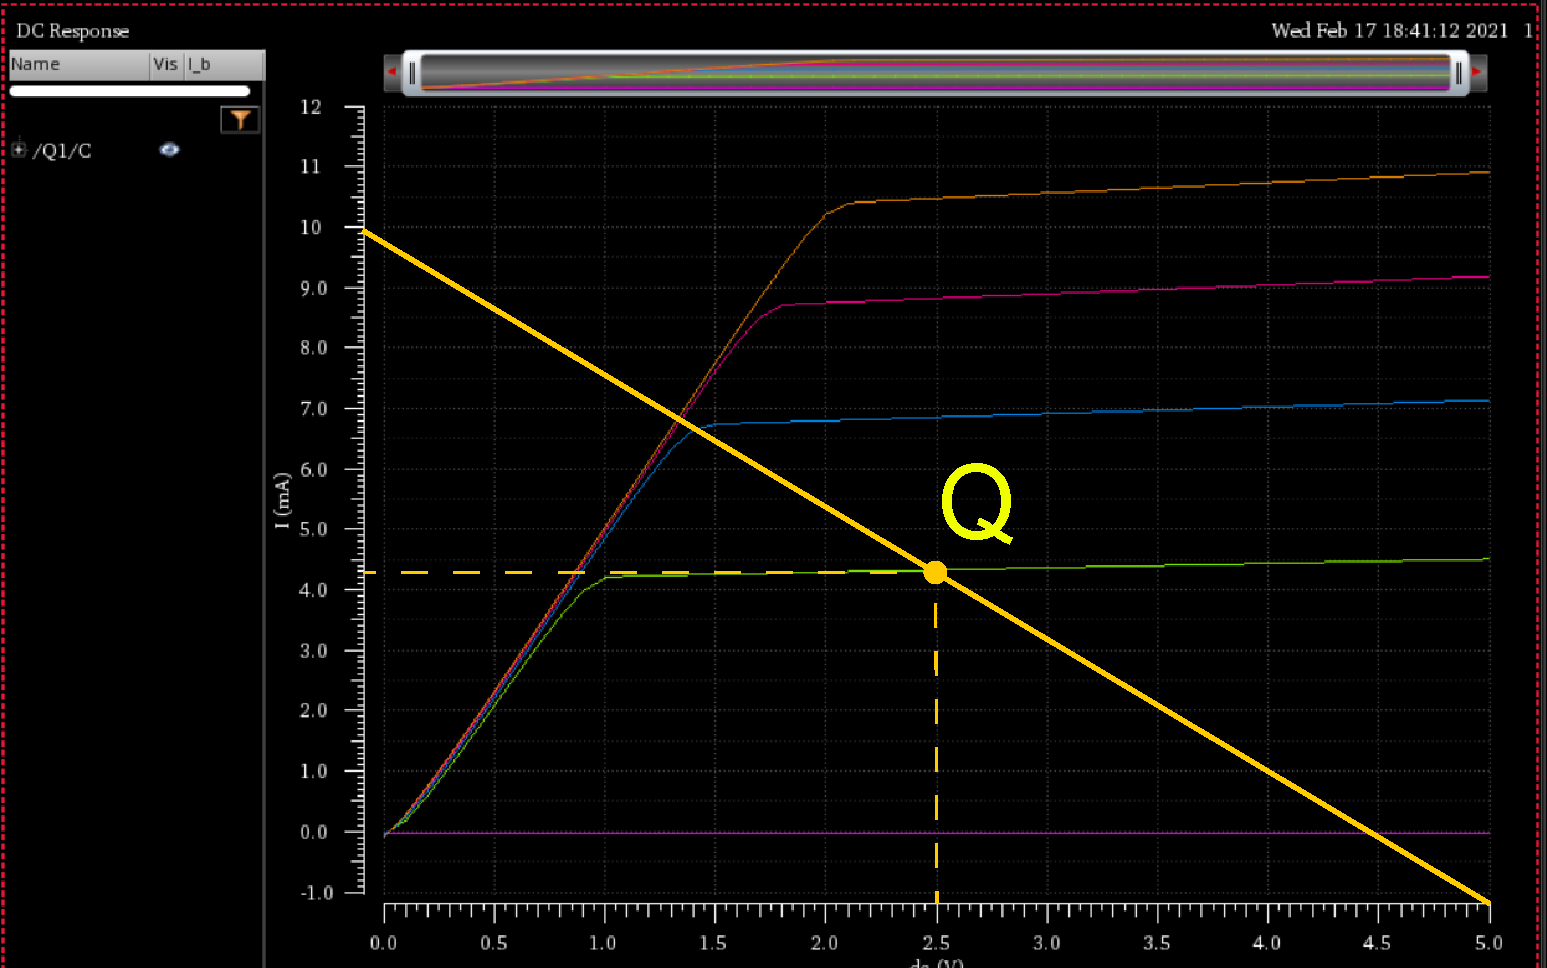
\includegraphics[width=0.8\linewidth]{1.png}}
\caption{Еквівалентна схема $Т_y$ з каналом $W_{\text{экв.}}=3W$.}
\label{ris1}
\end{figure}

\begin{figure}[h]
\center{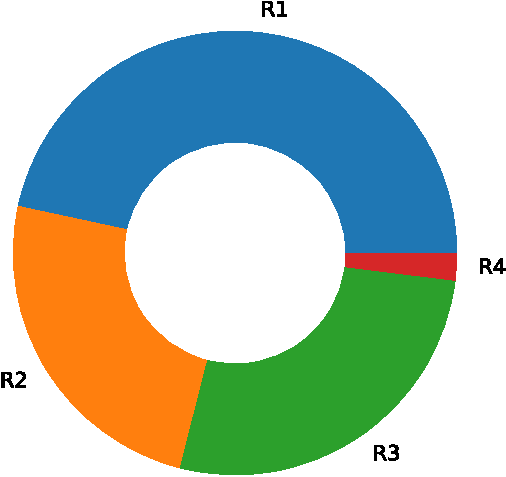
\includegraphics[width=0.8\linewidth]{2.png}}
\caption{Схема дослідження.}
\label{ris2}
\end{figure}

\begin{center}2.2.Таблиці\\ \end{center}
%---------------------------------------------------------------------------------------------------------------------------------------------------------------------------------
\newpage

Табл. 1: Сімейство вихідних характеристик керуючого МДН-транзистора\\

\begin{tabular}{|l|l|c|c|c|c|c|c|c|c|c|c|}
\hline  {$U_{3}=4,5$} & $U_{c}, B$ & 0 & 0,1 & 0,2 & 0,3 & 0,4 & 0,5 & 0,7 & 0,9 & 1,2 & 1,5 \\
\cline { 2 - 12 } & $I_{c l}, \text{мА}$ & 120 & 170 & 185 & 195 & 205 & 220 & 240 & 265 & 285 & 30\\
\hline
\end{tabular}
\vspace{1cm}

\begin{tabular}{|c|c|c|c|c|c|c|c|c|c|c|c|c|c|c|}
\hline$U_{3}=5$ & $U_{c},$ & 0 & 0,1 & 0,2 & 0,3 & 0,4 & 0,5 & 0,6 & 0,7 & 0,8 & 0,9 & 1 & 1,2 & 1,5 \\
\cline { 2 - 15 }& $I_{c l},$ & 60 & 85 & 110 & 140 & 162 & 180 & 198 & 215 & 239 & 245 & 255 & 275 & 295\\
\hline
\end{tabular}
\vspace{1cm}

\begin{tabular}{|l|l|c|c|c|c|c|c|c|c|c|c|}
\hline  {$U_{3}=5,5 B$} & $U_{c}, B$ & 0 & 0,1 & 0,2 & 0,3 & 0,4 & 0,5 & 0,6 & 0,7 & 0,8 & 0,84 \\
\cline { 2 - 12 } & $I_{c l}, \text{мА}$ & 15 & 65 & 105 & 140 & 170 & 200 & 225 & 265 & 290 & 300 \\
\hline
\end{tabular}
\vspace{1cm}

\begin{tabular}{|c|l|c|c|c|c|c|c|c|c|}
\hline  {$U_{3}=6 B$} & $U_{c}, B$ & 0 & 0,1 & 0,2 & 0,3 & 0,4 & 0,5 & 0,6 & 0,66 \\
\cline { 2 - 10 } & $I_{c l}, \text{мА}$ & 30 & 70 & 115 & 160 & 200 & 240 & 280 & 300 \\
\hline
\end{tabular}
\vspace{1cm}

\begin{tabular}{|l|l|c|c|c|c|c|c|c|}
\hline  {$U_{3}=6,5 B$} & $U_{c}, B$ & 0 & 0,1 & 0,2 & 0,3 & 0,4 & 0,5 & 0,55 \\
\cline { 2 - 9 } & $I_{c l}, \text{мА}$ & 35 & 85 & 140 & 180 & 235 & 285 & 300\\
\hline
\end{tabular}
\vspace{1cm}

\begin{tabular}{|l|l|c|c|c|c|c|c|}
\hline  {$U_{3}=7 B$} & $U_{c}, B$ & 0 & 0,1 & 0,2 & 0,3 & 0,4 & 0,5 \\
\cline { 2 - 8 } & $I_{c l}, \text{мА}$ & 40 & 90 & 145 & 200 & 255 & 300\\
\hline
\end{tabular}
\vspace{1cm}

\begin{tabular}{|c|l|c|c|c|c|c|c|c|c|c|}
\hline  {$U_{3}=7,5$} & $U_{c}, B$ & 0 & 0,1 & 0,15 & 0,2 & 0,25 & 0,3 & 0,35 & 0,4 & 0,44 \\
\cline { 2 - 11 } & $I_{c l}, \text{мА}$ & 30 & 105 & 130 & 165 & 190 & 220 & 250 & 275 & 300 \\
\hline
\end{tabular}
\vspace{1cm}

\newpage
Табл. 2: Передавальні характеристики МДН інтегрального інвертора для різних видів навантажень. Умови вимірювань: $E_{\text {ж}}=-15 B$.
\begin{figure}[h]
\center{\includegraphics[width=0.6\linewidth]{tab2.png}}
\end{figure}


\newpage
\begin{center}3.Формули та Розрахунки\\ \end{center}

Для початку знайду крутизну характеристики, диференційний опір та граничний кофіцієнт підсилення за напругою відповідно:
\begin{align}\label{q1}
  S = \dfrac{\triangle I_C}{\triangle U_{\text{3}}}
\end{align}
\begin{align}\label{q2}
  r_i = \dfrac{\triangle U_{BC}}{\triangle I_{C_2}}
\end{align}
\begin{align}\label{q3}
  K_U = S\cdot r_i
\end{align}


Беру значення з точок 3 та 4 і пiдставляю у формулу \ref{q1}, отримую
(при урахуванні що $\triangle U_{\text{СВ}} = const, \triangle U_{\text{З}} = const, \triangle U_{\text{З}} = 5,5 B$ відповідно у фомулах \ref{q1}, \ref{q2} та \ref{q3})\\

Тоді
\FPeval\s{round( (((235-200)*10^{-6})/0.5):8 )}

\begin{align*}
  S = \dfrac{(230-200)\cdot10^{-6}}{0,5} = \FPprint{s} = 70 \dfrac{\text{ мкА}}{B}
\end{align*}
%\noindent{\color{red} \rule{\linewidth}{1mm} }

\FPeval\ri{round((0.1/(30*10^{-6})):2) }
\begin{align*}
  r_i = \dfrac{0.1}{30\cdot 10^{-6}} =\FPprint{ri} = 3,3\text{ кОм}
\end{align*}


\FPeval\ku{round( ( s*ri ):2 )}
\begin{align*}
  K_U = S\cdot r_i = \FPprint{ku}
\end{align*}

Тепер користуючись рис.\ref{graf2} знайду коефіцієнти передачі для кожної перехідної характеристики і потім методом
трикутника знайду динамічний коефіцієнт підсилення для кожного із трьох типів
навантаження $\left(K = \dfrac{\triangle U_C}{\triangle U_3} \right)$

Як я зрозумів, то у мене недостатньо виміряних значень, тому я  не можу побудувати \\ пологу частину ВАХ і визначити навантажувальні характеристики...
\FPeval\a{8-6}

\FPeval\tn{round(a/(3.5-3.1):2)}
\begin{align*}
  K_{Tn} = \dfrac{8-6}{3,5-3,1} = \FPprint{tn}
\end{align*}

\FPeval\ty{round(a/(6.5-5.5):2)}
\begin{align*}
  K_{Ty} = \dfrac{8-6}{6,5-5,5} = \FPprint{ty}
\end{align*}


\FPeval\rn{round(a/(7.8-7):2)}
\begin{align*}
  K_{Rn} = \dfrac{8-6}{7,8-7} = \FPprint{rn}
\end{align*}




















\newpage
\begin{center}4.Графіки\\ \end{center}
Будую сімейство використовуючи дані з Таб.1.

\begin{figure}[h]
\center{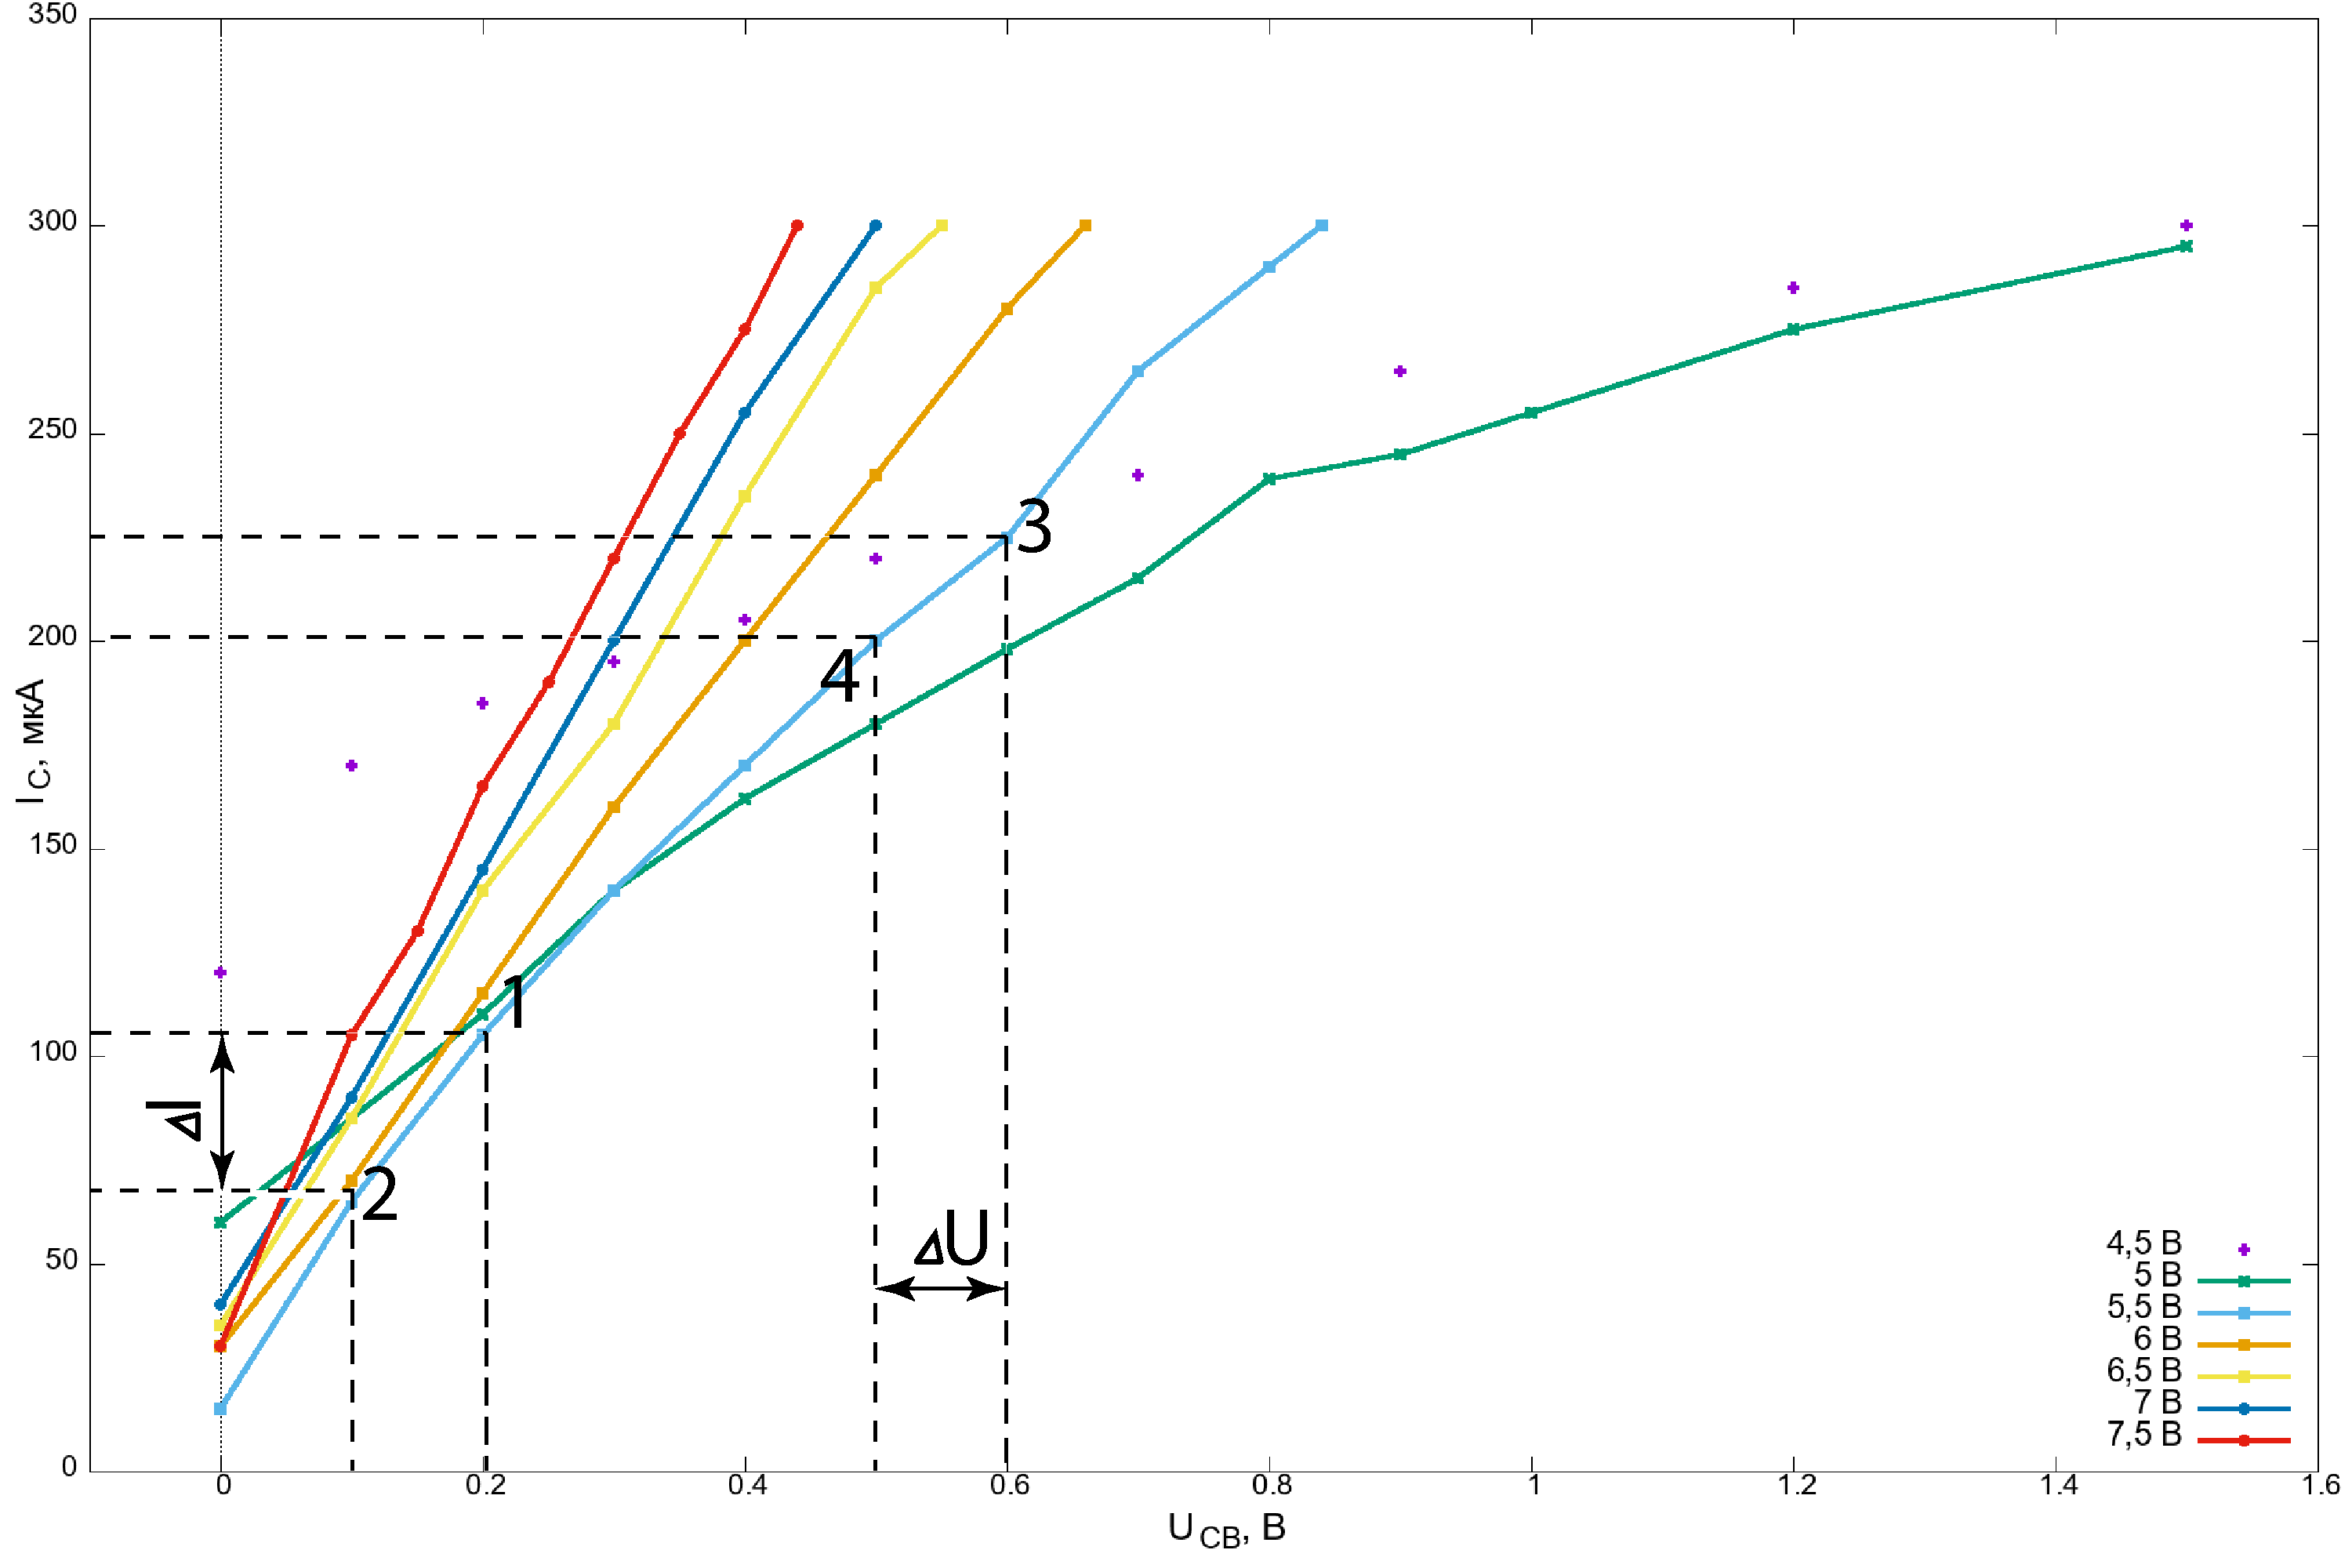
\includegraphics[width=1\linewidth]{d1.pdf}}
\caption{Вихідні характеристики транзистора.}
\end{figure}
Виміри для Uз = 4,5 В щось не дуже сходяться з теоретично можливими, тому я виключив їх з розрахунків.

\begin{figure}[h]
\center{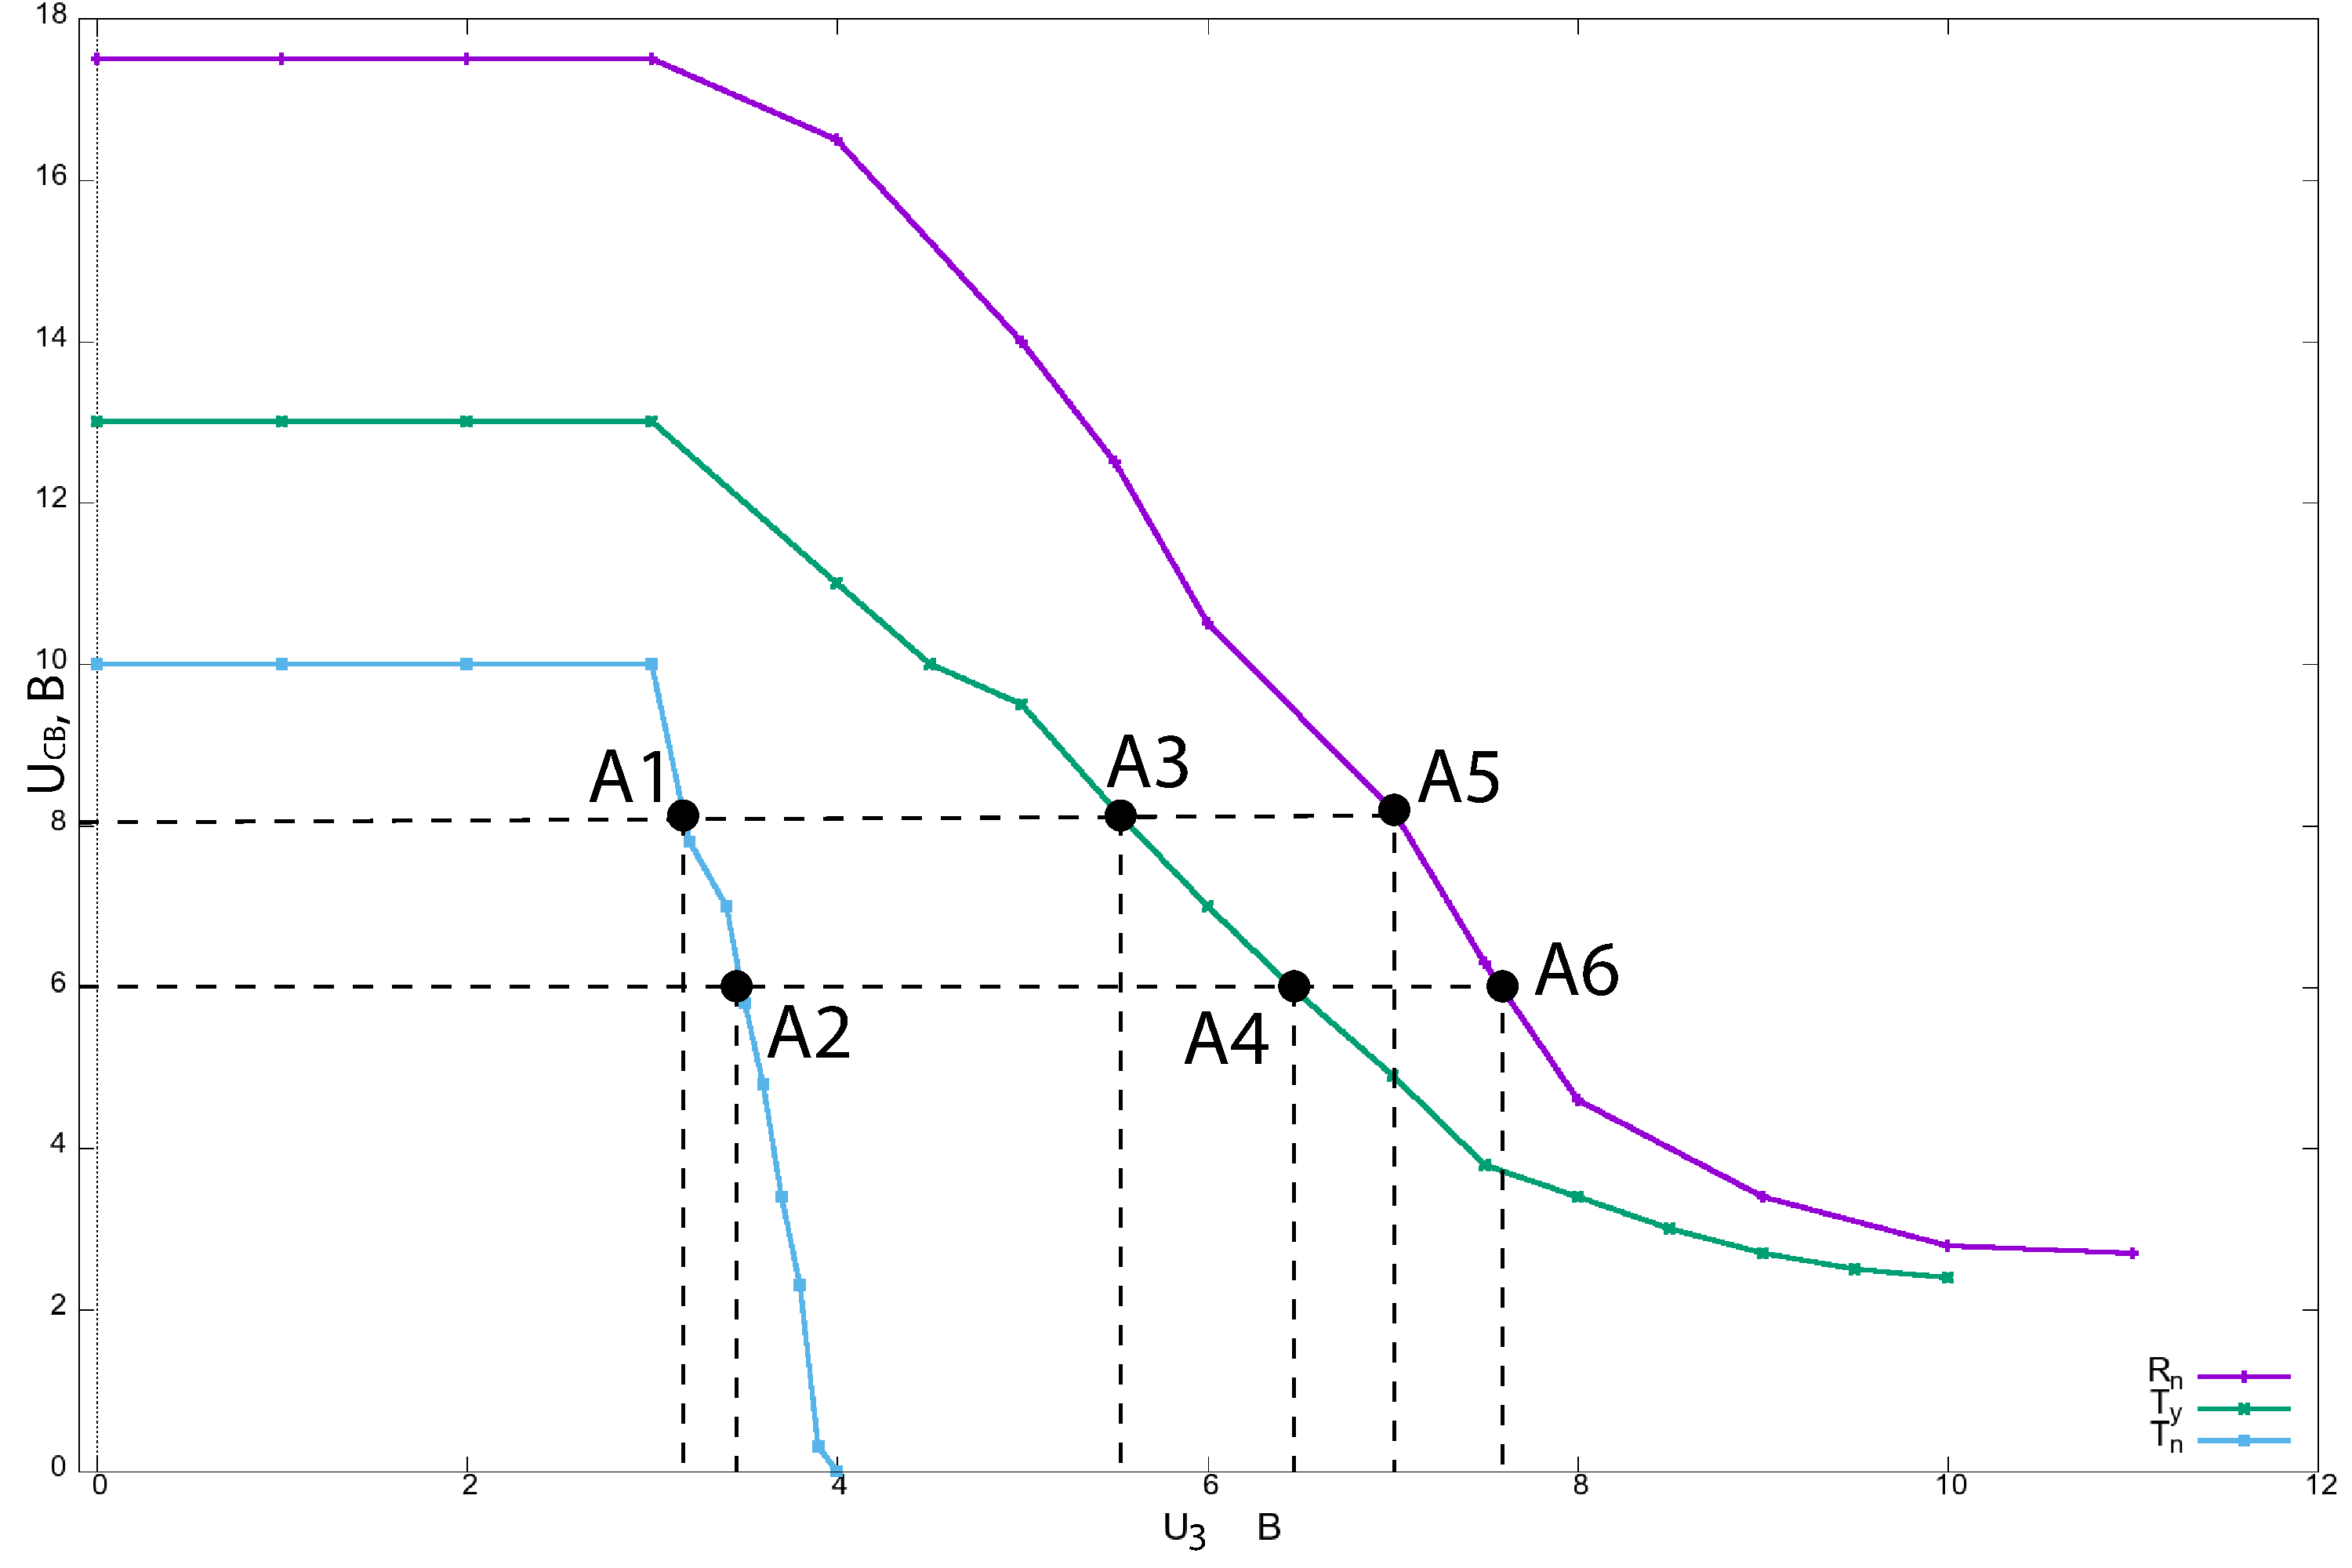
\includegraphics[width=1\linewidth]{d2.pdf}}
\caption{Передавальна характеристика для трьох навантажень.}
\label{graf2}
\end{figure}




ж перехідних характеристик спадають, починаючи зі значення

\begin{figure}[h]
\center{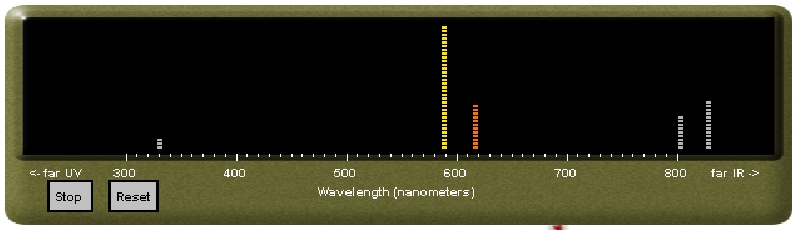
\includegraphics[width=0.8\linewidth]{3.png}}
\caption{Cтруктура КМОП інвертора.}
\end{figure}



\clearpage
\begin{center}5. Висновок\\ \end{center}
Виходячи з теореричних знань, можна сказати, що отримані на практиці ВАХ відповідають теоретичним припущенням, оскильки на всіх сімействах добре видна дилянка змини, а що стосується перехідних характеристик, то вони спадають, починаючи зі значення очевидного занченя, тобто з $U_{nop}$. Що стосується найкращого логічного елементу, то  на мою думку це буде зв'язка за транзистором $T_y$ оскільки він дає найбільший коефіцієнт передачі.




\end{document}
